% vim: set spell spelllang=en tw=100 et sw=4 sts=4 :

\documentclass{llncs}

% \usepackage{showframe}

\usepackage{complexity}
\usepackage{hyperref}
\usepackage{microtype}
\usepackage{cleveref}                  % no need to type Figure etc
\usepackage{xcolor,colortbl}

\usepackage{todonotes}
\usepackage{booktabs}

% lncs style
\crefname{algocf}{Algorithm}{Algorithms}
\Crefname{algocf}{Algorithm}{Algorithms}
\crefname{figure}{Fig.}{Figs.}
\Crefname{figure}{Fig.}{Figs.}
\crefname{table}{Table}{Tables}
\Crefname{table}{Table}{Tables}
\crefname{proposition}{Proposition}{Propositions}
\Crefname{proposition}{Proposition}{Propositions}

\title{Portfolios of Subgraph Isomorphism Algorithms}

\author{
    Lars Kotthoff\inst{1}
    \and Ciaran McCreesh\thanks{This work was supported by the Engineering
        and Physical Sciences Research Council [grant number EP/K503058/1]}\inst{2}
    \and Patrick Prosser\inst{2}
    \and Christine Solnon\inst{3}}

\institute{
    University of British Columbia, Vancouver, Canada
    \and University of Glasgow, Glasgow, Scotland
    \and INSA-Lyon, LIRIS, UMR5205, F-69621, France}

\begin{document}

\maketitle

\begin{abstract}
Subgraph isomorphism is a computationally challenging problem with lots of important practical
applications, for example in computer vision, biochemistry, and model checking. There are a number
of state-of-the-art algorithms for solving it, each of which has its own performance
characteristics. As with many other hard problems, the single best choice of algorithm overall is
rarely the best algorithm for each instance. We develop a portfolio approach that leverages novel
features to characterise subgraph isomorphism problems to dynamically decide which algorithm to use
on a per-instance basis. We demonstrate significant performance improvements on a large set of hard
benchmark problems. In addition, we show how algorithm selection models can be leveraged to gain new
insights into what affects the performance of an algorithm.
\end{abstract}

\section{Introduction}

The subgraph isomorphism problem is to find an injective mapping from vertices of a small
\emph{pattern} graph to vertices of a large \emph{target} graph which preserves adjacency. This
\NP-complete problem has lots of important practical applications, for example in computer vision,
biochemistry, and model checking. There exist various exact algorithms, which have been compared on
a large benchmark in  \cite{McCreesh:2015}. These experiments indicated that the single best
algorithm depends on the CPU time limit considered: for very small (resp. larger) CPU time limits,
VF2 \cite{Cordella:2004} (resp. the Glasgow algorithm \cite{McCreesh:2015}) has better success
rates. Furthermore, they also showed us that on an instance by instance basis, other algorithms may
become better.

In this paper, we report experimental results on a larger set of 8 algorithms, including new
variants, and a larger benchmark. We show that 5 of these algorithms are single best algorithms,
depending on the CPU time limit considered, and that combining preprocessing with an algorithm
selection on an instance by instance basis allows us to achieve better overall performance than any
single algorithm.

\section{Per-Instance Algorithm Selection}

The per-instance algorithm selection problem~\cite{rice_algorithm_1976} is to select from an
algorithm portfolio~\cite{huberman_economics_1997,gomes_algorithm_2001} the one expected to perform
best on a given problem instance. Algorithm selection systems usually build machine learning models
of the algorithms or the portfolio they are contained in to forecast which algorithm to use in a
particular context. Using the model predictions, one or more algorithms from the portfolio are
selected to be run sequentially or in parallel.

Here, we consider the case where exactly one algorithm is selected for solving the problem. One of
the most prominent and successful systems that employs this approach is
SATzilla~\cite{xu_satzilla_2008}, which defined the state of the art in SAT solving for a number of
years. Other application areas include constraint solving~\cite{omahony_using_2008}, the travelling
salesperson problem~\cite{kotthoff_improving_2015}, and AI planning~\cite{seipp_learning_2012}.
The interested reader is referred to a recent survey~\cite{kotthoff_algorithm_2014} for additional
information on algorithm selection.

\subsection{Subgraph isomorphism algorithms}

We consider the following exact subgraph isomorphism
algorithms: VF2 \cite{Cordella:2004}, which is a simple backtracking search algorithm, especially
fast on trivially satisfiable instances; LAD \cite{Solnon:2010}, which does very strong reasoning
based on local all different redundant constraints; and the Glasgow algorithm \cite{McCreesh:2015},
which does an expensive preprocessing pass once, followed by weaker reasoning during search.

The Glasgow algorithm has a parameter, which controls the lengths of paths used when reasoning about
non-adjacent vertices.  In experiments reported in \cite{McCreesh:2015}, the choice of paths of
length 3 was used as a reasonable compromise---longer paths lead to prohibitively expensive
preprocessing on larger, denser instances. This is often not the best choice on an instance by
instance basis: sometimes path-based reasoning gives no benefit at all, sometimes considering only
paths of length 2 suffices, occasionally paths of length 4 are helpful, and even looking at paths of
length 3 is relatively expensive on some graphs. Therefore, in this new study, we consider 4
different instances of the Glasgow algorithm, with path lengths varying from 1 to 4.

We also introduce two new variants of LAD. The first variant is a weaker LAD filtering (called LAD
preprocessing) which is applied once, without performing a backtracking search, and detects
inconsistencies on many instances: For each pattern node $u$, we check that there exists at least
one target node $v$ such that for each neighbor $u'$ of $u$ there exists a different neighbor $v'$
of $v$ such that the degree of $u'$ is smaller than or equal to the degree of $v'$. LAD
preprocessing is an incomplete algorithm as it can only detect inconsistency of some instances: when
it does not detect inconsistency, the instance may either be consistent or not. The time complexity
of LAD preprocessing is ${\cal O}(n(n'+p'))$ where $n$ and $n'$ are the number of pattern and target
nodes, respectively, and $p$ is the number of target edges.

The second variant of LAD is called new LAD and it is stronger than the default LAD introduced in
\cite{Solnon:2010}. It combines LAD filtering with new invariant properties borrowed from SND
\cite{Audemard:2014}. The idea is to label each edge $(u,v)$ with the number of paths of length 2
between $u$ and $v$, and each node $u$ with the number of cycles of length 3 passing through $u$,
and to add the constraint that the label of a pattern node (resp. edge) must be smaller than or
equal to the label of its associated target node (resp. edge).

\subsection{Problem instances}

We consider 5725 instances, which are available in a simple text
format\footnote{\url{http://liris.cnrs.fr/csolnon/SIP.html}}. These instances are grouped into 12
classes.

\begin{itemize}
\item Class 1 contains randomly generated scale-free graphs \cite{}.
\item Classes 2 and 3 contain various kinds of graphs coming from \cite{}: class 2 contains small
    instances generated from the 50 first graphs of the benchmark, whereas class 3 contains larger
    instances where pattern graphs are coming from class 2, and target graphs are coming from the
    next 50 graphs of the benchmark.
\item Classes 4 to 8 contain randomly generated graphs coming from \cite{GraphDatabase}:
    bounded-degree graphs for classes 3 and 4, regular meshes for classes 5 and 6, and random graphs
    with uniform edge probabilities for class 7.
\item Classes 9 and 10 contain instances coming from images \cite{}.
\item Class 11 contains instances coming from meshes modeling 3D objects \cite{}.
\item Class 12 contains random graph instances belonging to the phase transition.
\end{itemize}

Note that Classes 3 and 12 were not considered in the previous experimental study reported in \cite{McCreesh:2015}.

\subsection{Features}

For both the pattern and the target graph, we consider the number of vertices, edges and loops, the
mean and maximum degree, the density, whether or not every vertex has same degree, whether or not
the graph is connected, the mean and maximum distances between all pairs of vertices, and the
proportion of vertex pairs which are distance at least 2, 3 and 4 apart. We also consider the number
of variable-value assignments removed by LAD preprocessing in absolute terms, as a percentage, and
the minimum and maximum on a per-variable basis.  This gives us a total of 30 features.

\subsection{Experimental Setup}

We measured runtimes on machines with Intel Xeon E5-2640 v2 CPUs and 64GBytes RAM, running
Scientific Linux 6.5. We used the C++ implementation of the Glasgow algorithm \cite{McCreesh:2015},
the C implementation of LAD \cite{Solnon:2010}, and the VFLib C implementation of VF2
\cite{Cordella:2004}. Software was compiled using GCC 4.9. Each problem instance was run with a
timeout of $10^8$ milliseconds (a little over a day).

\subsection{Algorithm Selection approach}

We apply two static steps to each instance before solving it. First, the computation of the LAD
features can detect unsatisfiability of an instance. If an instance is identified as unsatisfiable,
we do not process it further.  Second, we run the VF2 solver for 0.05 seconds. This solves easy
instances without the overhead of running algorithm selection and avoids potentially making
incorrect solver choices.

Computing the LAD features detects unsatisfiability on 1919 instances. Running VF2 for 0.05 seconds
removes a further 1470. We are left with 2336 hard instances that we consider for algorithm
selection.

To decide which solver to run on the remaining instances, we use LLAMA~\cite{kotthoff_llama_2013}.
In preliminary experiments, we identified random forest regression to predict the performance
difference between pairs of algorithms, with the best algorithm identified as the one with the best
cumulative performance difference over all pairs, as the best approach. We make no claims that this
is the overall best approach.

The data we use in this paper is available as Aslib scenario GRAPHS-2015.

\section{Experimental Results}

Table~\ref{tab:res} shows the performance of our algorithm selection approach, compared to two
baselines. The virtual best solver is the oracle predictor that, for each instance, chooses the best
solver from our portfolio. This is the upper bound of what an algorithm selection approach can
achieve. The single best solver is the one solver from the portfolio that has the overall best
performance across the entire set of instances. We consider it a lower bound on performance.

\begin{table}[ht]
\centering
\begin{tabular}{lr}
  \toprule
& mean runtime\\
  \midrule
virtual best & 5822.809\\
  single best & 7788.719\\
  LLAMA & 6509.947\\
   \bottomrule
\end{tabular}
\vspace{1ex}
\caption{Algorithm selection performance on reduced set of 2336
instances.}\label{tab:res}
\end{table}

We are able to close more than 60\% of the performance gap between the single
best and the virtual best solver, our lower and upper bounds. For comparison, we
show the results achieved on the entire set of instances without
unsatisfiability detection and presolving in Table~\ref{tab:resfull}. We achieve
similar results with more than 58\% of the gap between the single best and the
virtual best closed.

\begin{table}[ht]
\centering
\begin{tabular}{lr}
  \toprule
& mean runtime\\
  \midrule
virtual best & 2375.913\\
  single best & 3177.569\\
  LLAMA & 2706.749\\
   \bottomrule
\end{tabular}
\vspace{1ex}
\caption{Algorithm selection performance on the full set of 5725
instances.}\label{tab:resfull}
\end{table}

Figure~\ref{fig:scatter} shows detailed results for each of the 2336 instances
in the reduced set. Our algorithm selection approach is by no means able to
identify the best solver on a majority of instances, although we are able to
achieve performance improvements overall. There seems to be no particular
pattern as to where algorithm selection performs well and where it fails.

\begin{figure}[!ht]
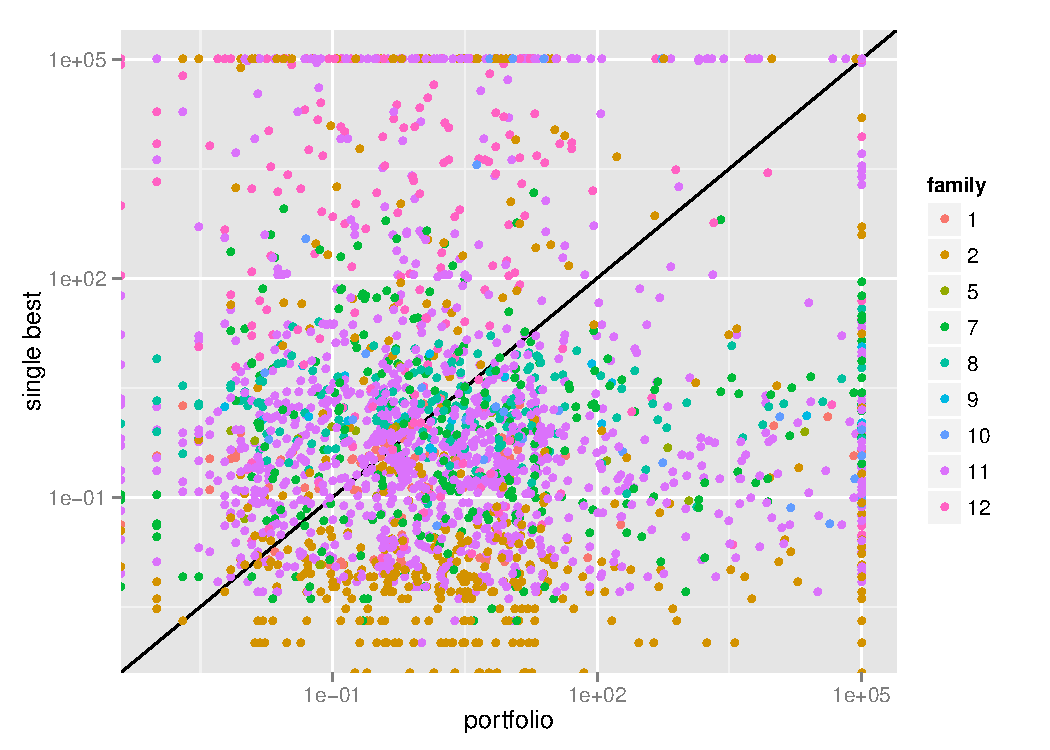
\includegraphics[width=\textwidth]{figures/perfScatter}
\caption{Single best algorithm vs.\ portfolio performance on all instances by
family. Points above the diagonal indicate that the portfolio achieved better
performance, while the single best solver was better on instances below the
diagonal.}
\label{fig:scatter}
\end{figure}

Figure~\ref{fig:portfolio-ecdf} shows the cumulative density function for the
individual solvers, the virtual best solver, and the LLAMA portfolio. The
virtual best solver clearly dominates with a significant margin to the next
best. VF2 is far below all other solvers. The portfolio does not perform well
for instances that can be solved quickly because of the overhead incurred
through feature computation. As the instances become more difficult to solve,
its performance improves. For instances that take more than 1,000 seconds to
solve, the portfolio eclipses any individual solver and closes most of the gap
to the virtual best solver.

\begin{figure}[!ht]
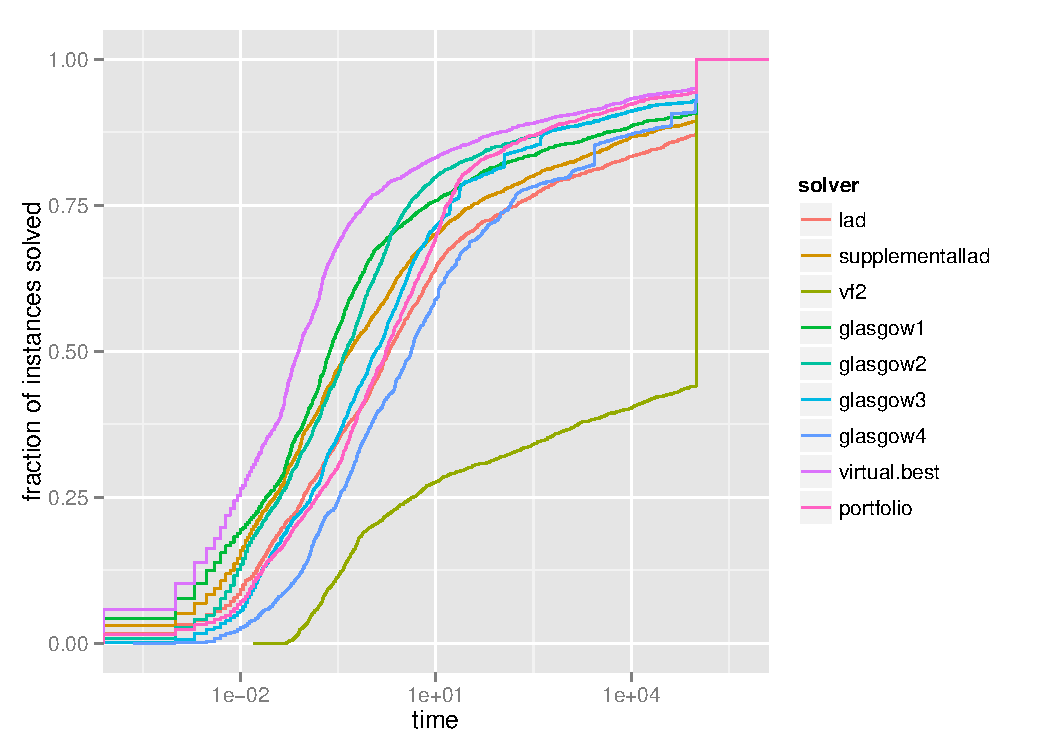
\includegraphics[width=\textwidth]{figures/portfolio-ecdf}
\caption{Empirical cumulative density function of solvers, virtual best solvers,
and the LLAMA portfolio.}
\label{fig:portfolio-ecdf}
\end{figure}

\begin{table}[t]
\begin{center}
\begin{tabular}{|c||r||r|r|r||r|r|r|r||r|r|}
\hline
$t$ & VF2 & \multicolumn{3}{c||}{LAD} & \multicolumn{4}{c||}{Glasgow}& VBS & $\delta$\\
&&pre&def&new&1&2&3&4&&\\\hline
$10^0$ & 300 &  \cellcolor{blue!25}1126 & 661 & 599 & 386 & 95 & 39 & 12 & 1132 & 6\\\hline
$10^1$ & 1699 & 1858 & 2101 &  \cellcolor{blue!25}2287 & 2061 & 1215 & 455 & 208 & 3388 & 101\\\hline
$10^2$ & 2834 & 1912 & 3376 & 3708 &  \cellcolor{blue!25}3943 & 3344 & 2295 & 1329 & 4636 & 693\\\hline
$10^3$ & 3458 & 1918 & 4233 & 4531 &  \cellcolor{blue!25}4908 & 4763 & 4262 & 3426 & 5170 & 262\\\hline
$10^4$ & 3701 & 1919 & 4888 & 5025 & 5156 &  \cellcolor{blue!25}5253 & 5022 & 4408 & 5332 & 79\\\hline
$10^5$ & 3850 & 1919 & 5108 & 5193 & 5301 &  \cellcolor{blue!25}5377 & 5292 & 5082 & 5434 & 57\\\hline
$10^6$ & 3977 & 1919 & 5244 & 5307 & 5386 &  \cellcolor{blue!25}5452 & 5451 & 5235 & 5500 & 48\\\hline
$10^7$ & 4082 & 1919 & 5336 & 5414 & 5458 & 5517 &  \cellcolor{blue!25}5518 & 5425 & 5567 & 49\\\hline
$10^8$ & 4191 & 1919 & 5423 & 5479 & 5508 &  \cellcolor{blue!25}5561 & 5560 & 5554 & 5608 & 47\\\hline
\end{tabular}
\end{center}
\caption{Number of solved instances at different CPU time limits: Each line displays a time limit
$t$ (in milliseconds) followed by the number of instances solved within this time limit by VF2, LAD
preprocessing, default LAD, and new LAD, Glasgow with  the lengths of paths limited to 1, 2, 3 and
4, and the VBS. The best single algorithm is highlighted in blue, and the difference between VBS and
single best if displayed in the last column ($\delta$).\label{expTime}}
\end{table}

Table \ref{expTime} displays the number of instances solved at different CPU time limits, ranging
from 1 to $10^8$ milliseconds. It shows us that the best single solver depends on the time limit
considered. Simple approaches like LAD preprocessing and VF2 are able to solve easy instances very
quickly, in a few milliseconds. However, they are not able to solve harder instances: LAD
preprocessing is an incomplete approach which can only detect rather trivial unconsistencies; VF2
performs a basic backtracking search and is very fast on easy instances, because it does not compute
expensive invariants. Default LAD, new LAD, and the Glasgow algorithms solve more instances than VF2
and LAD preprocessing when considering longer time limits: 10 ms for default and new LAD and Glasgow
1, and 100 (resp. 1000 and 10000) ms for Glasgow 2 (resp. 3 and 4). The Virtual Best Solver (VBS),
which considers the best algorithm for each instance separately, obtains much better results,
showing us that the algorithms have complementary performance. The difference between VBS and single
best (column $\delta$ of Table \ref{expTime}) is more particularly important for rather small CPU
time limits. In particular, VBS solves 693 more instances than the single best (Glasgow 1) when the
limit is 100 ms. In many applications, it is important to have the fastest possible algorithm. For
example, in pattern recognition applications, we often have to solve subgraph isomorphism problems
for a very large number of graphs (in order to find a pattern image in a large database of target
images, for example), so that having an algorithm that is able to solve an instance in 100 ms
instead of 1000 ms makes a big difference. Therefore, it is important to select the best algorithm
for each instance.

Table \ref{expClass} shows us that we cannot reasonably split things up based upon which class
instances are coming from, unlike SAT. For all classes, there are always at least 2 algorithms which
are the best for at least one instance of the class. In particular, for classes 2 and 3, each
algorithm is the best for at least one instance (except Glasgow 4 for Class 2).

\begin{table}
\begin{center}
\begin{tabular}{|c||r||r|r|r||r|r|r|r|}
\hline
Class & VF2 & \multicolumn{3}{c||}{LAD} & \multicolumn{4}{c|}{Glasgow}\\
&&pre&def&new&1&2&3&4\\\hline
1\\\hline
2\\\hline
3\\\hline
4\\\hline
5\\\hline
6\\\hline
7\\\hline
8\\\hline
9\\\hline
10\\\hline
11\\\hline
12\\\hline

\end{tabular}
\end{center}
\caption{Number of times each algorithm is best, for each class.\label{expClass}}
\end{table}

Table 3 shows the performance of our algorithm selection approach, compared to the VBS (which is the
upper bound of what an algorithm selection approach can achieve), and the single best solver, at
different CPU time limits (the single best corresponds to results highlighted in blue in Table 1).
Comment Table 3: Mean runtime but also number of solved instances at different CPU time limits.
Logically, LLAMA may solve less instances than single best for small time limits because it spends
time to compute features and choose a solver, but it should be better for larger time limits...

\begin{table}
\begin{tabular}{|l|r|rrrrrrrrr|}
&mean & \multicolumn{9}{c|}{Number of solved instances}\\
&runtime & $10^0$ &  $10^1$ &  $10^2$ &  $10^3$ &  $10^4$ &  $10^5$ &  $10^6$ &  $10^7$ &  $10^8$\\\hline
VBS & 2375.9 & 1132 & 3388 & 4636 & 5170 & 5332 & 5434 & 5500 & 5567 & 5608\\\hline
Single best & 3177.6 & 1126 & 2287 & 3943 & 4908 & 5253 & 5377 & 5452 & 5518 & 5561\\\hline
LLAMA & 2706.3\\\hline
\end{tabular}
\caption{}
\end{table}

Add Figure 1 which compares single best at $10^8$ ms (Glasgow 2) with LLAMA ?

\section{Conclusion and Future Work}

Mention parallel, directed, labelled in here briefly.

\bibliographystyle{splncs}
\bibliography{paper}

\end{document}

